\epigraph{\textit{"The first rule is to never lose money. The second rule is to never forget the first one."}}{Warren Buffett} 

\paragraph{}

Over this chapter, the \textbf{financial study} is going to be performed. The costs and the profits will be analyzed, and some important figures will be acquired. 

Moreover, some other important considerations, such as social and security issues or environmental impact will be studied too.

\chapter{Financial Study}

The different departments have estimated the main costs of the project. It is high time to start performing a deep analysis on the economical solvency of the project. The analysis carried on will be of 12 years. The decision of this amount of years has been done taking into account that every 5 years there is a re-launching of the whole constellation, which means that in year 5, 10, 15... a considerable increase in the costs is to be done. In order to have a good view of the whole project, it has been decided that at least two full cycles had to appear complete (years 0 to 4 and 5 to 9) and also to see the tendency it was recommended to add some more time. This is the reason why the studied is carried on for 12 years. 

Up to this point, it is important to determine how this product will be sold, so as to quantify the benefits of the project and be able to determine some figures such as the Pay Back Time or the Net Present value, and be able to make some conclusions. 

\section{Selling the product}

The aim of the project is to be able to sell to the customers the chance of both sending and receiving data from satellites. Therefore, it seems logic that the price of the product has to be somehow related to the amount of data passed on. Then, there will be a price for every Mbit, either sent or received. 

From the Communications Department, there is a limitation of 3 Ground Stations operating, and each one can carry up to 25 Mbits/second. Accepting that those Ground Stations will fully operating the whole year, and calculating the amount of seconds that there are in a normal year:
\begin{equation}
365 \cdot 24 \cdot 60 \cdot 60 = 31536000 s
\end{equation}
It can be easily calculated the amount of Mbits that Astrea Constellation is able to either send or receive:
\begin{equation}
31536000 \cdot 75 = 2365200000 Mbits
\end{equation}
This means that no more than 2365200000 Mbits can be sold. This is the maximum supply.

But how can the demand be estimated? There is a need to make assumptions. 

\subsection{Estimation of demand}

\subsubsection{Universities}

Firstly, it has been thought that the service offered has great academic interests. In fact, any student could build a satellite with a certain payload, send it to space and then receive data from the satellite at any time thanks to Astrea constellation. 
\newline
\newline
In order to study the possible demand of Mbits, an estimation of the possible universities that would want to use the services has been done. Fortunately, the list of universities that offer studies in the aerospace field goes back a total of 400 schools approximately. Nevertheless, it is highly improbable that all those colleges become clients because not all universities have the same sources or interests. Therefore, the following list presents the number of existing colleges having an aerospace degree in each continent.

	\begin{table}[!h]
	\begin{center}
	\begin{tabular}{|c|c|}
	\bf{Continent} & \bf{Number of Universities}\\
	\hline 
	Europe & 124\\
	\hline 
	Asia & 138\\
	\hline 
	North America &  97\\
	\hline
	 South America & 18\\
	\hline 
	Australia & 8\\
	\hline 
	Africa & 12\\
	\end{tabular}
	\end{center}
	\caption{Table. List of Universities with Aerospace Degrees}
	\end{table} 	

By analyzing this information, it can be determined that the continents with countries with higher PIB have more colleges interested in the space field. It is noticed that Asia is the continent with more colleges because, even if it is mostly poor, it is so big that it has rich countries such as Japan, Korea or China and the United Arab Emirates. Moreover, Europe and North America are not so extensive but have a higher aerospace culture and interest. 
\newline
\newline
On the basis the service is affordable for many prestigious colleges and it permits to provide their students with the chance to improve their knowledge by doing their own experiments, it has been estimated that about 50 universities could end up contracting Astrea's service in the next years. If it is assumed that each university would be interested in sending or receiving a total of 19710000 Mbits anually, therefore the number of Mbits for universities, anually, will be of 98550000 Mbits.

\subsubsection{Particular customers}
Another extremely important sector of clients are the private ones. It is harder to make an assumption on the number of Mbits consumed by this sector. Nevertheless, some figures are needed in order to perform a good feasibility study. 

According to the Union of Concerned Scientists of the United States of America, right now there are about 1500 satellites orbiting around the Earth. But every day space technology is more affordable and feasible, which leads to think that in the next years a good figure of satellites would be of roughly 2000. Therefore, there are two big groups of potencial clients, the ones already orbiting and the ones who will be doing it soon enough.

Of the 1500 already existing satellites, it must be taken into account that they already have their own communication system. Astrea provides them a way of communicating with the satellites almost in real time, which is a great improvement, but as they already have their own method of communciating, they might not find so attractive this new company. Therefore, the demand is that of those 1500 satellites, about 50 would really be interested in using Astrea to send and receive data in real time, because they would really take good profit of it.

Of the 500 which are forecasted to be, it is easier that they are interested in Astrea, because they still have not determined the communication system of their satellite, and therefore they would really find interesting Astrea's service. As Astrea provides a very competitive price, it seems reasonable to think that a good percentage of those satellites would be interested. In order to be conservative, a 50\% of those would be potencial clients. This means that 250 full operating satellites would use Astrea, and assuming also than the average amount of data that those satellites would either send or receive anually is of 1971000 Mbits, the number of Mbits for particular clients, anually, will be of 492750000 Mbits.

It can be checked that the sum of the amounts of Mbits for universities and for particular clients, which is of 591300000
Mbits, is lower than the maximum amount of Mbits due to the 3 Ground Stations, which is of 2365200000 Mbits. There will not be problem of demand over capacity. 

\subsubsection{Demand}
Taking into account both the universities and the particular clients, and making a conservative assumption, the estimation of the demand, in Mbits, is of a fourth of the maximum capacity of Astrea, this is, 591300000 Mbits anually. Also, in order to simulate the unceirtainty of the company during the first years (as years pass, the company gets reputation and therefore its amount of clients also enlarges), a percentage is applied during the first years. This means that first year only a 75\% of the potential customers exposed before will be achieved, the second year a 80\%, and so on, until the sixth year, in which a 100\% is achieved. 

\subsection{Pricing the service}
The determination of the price is made upon the feasibility study, in order to get a reasonable Pay Back Time and benefit. Nevertheless, it is a fact that the fare of Astrea service must fulfill a condition: it has to be competitive. 

Comparing with some others similar services, in order to provide a competitive fare, it seems reasonable a price per Mbit of no more than 0.5 \euro per Mbit, as an upper tape.  


\section{Economic Feasibility Report}

In order to perform the analysis on the economical solvency of the project, next there is a table which contains the main costs of the project, as well as the numerical operations that allow to calculate some important financial parameters, such as the Net Present Value (NPV), the Internal Rate of Retorn (IRR), the Simple Pay Back Time (PBT), the Updated Pay Back Time (UPBT) and the Break Even Point (BEP). From this data, some conclusions will be drawn.

Firstly, though, there is need to take into account some costs that are not included in the other departments, and which are key to analyzing the costs and benefits. 
\subsection{Previous costs}
\subsubsection{Engineering hours}
The engineering hours, which were specified in the Project Charter, are again synthesized in the following table:

\begin{longtable}{ccc}
\toprule
\rowcolor[gray]{0.65}
    \textbf{Engineering hours budget} & \textbf{Hours} & \textbf{Labor cost (\euro)} \\
    \midrule
    \endhead
\hline
\rowcolor[gray]{0.85}
	MANAGEMENT &  &  \\ \hline
	Meetings documentation &  &  \\ \hline
	Meetings & 340 & 6800 \\ \hline
	Meetings preparation &  &  \\ \hline
	Agendas & 10 & 200 \\ \hline
	Minutes & 10 & 200 \\ \hline
	Task Tracking and scheduling &  &  \\ \hline
	Project Charter & 170 & 3400 \\ \hline
	Team tasks monitoring & 20 & 400 \\ \hline
	WBS and Gantt update & 10 & 200 \\ \hline
	\rowcolor[gray]{0.85}
	SATELLITE DEVELOPMENT &  &  \\ \hline
	Spacecraft subsystems & 180 & 3600 \\ \hline
	Payload &  &  \\ \hline
	Antenna & 40 & 800 \\ \hline
	PHDS & 50 & 1000 \\ \hline
	\rowcolor[gray]{0.85}
	ORBITAL DESIGN &  &  \\ \hline
	Constellation geometry & 220 & 4400 \\ \hline
	Orbit parameters &  &  \\ \hline
	General parameters & 120 & 2400 \\ \hline
	Drift & 100 & 2000 \\ \hline
	Legislation & 50 & 1000 \\ \hline
	\rowcolor[gray]{0.85}
	LAUNCH SYSTEMS &  &  \\ \hline
	Vehicle & 60 & 1200 \\ \hline
	Satellite deployer & 10 & 200 \\ \hline
	Replacement strategy & 100 & 2000 \\ \hline
	\rowcolor[gray]{0.85}
	OPERATION &  &  \\ \hline
	Communication protocol & 100 & 2000 \\ \hline
	Ground station & 80 & 1600 \\ \hline
	End of life strategy & 80 & 1600 \\ \hline
	\rowcolor[gray]{0.85}
	FINANCIAL PLAN &  &  \\ \hline
	Costs &  &  \\ \hline
	Fix &  &  \\ \hline
	Maintenance and cost analysis & 10 & 200 \\ \hline
	Insurance cost analysis & 15 & 300 \\ \hline
	Administration cost analysis & 15 & 300 \\ \hline
	Taxes cost analysis & 25 & 500 \\ \hline
	Variable &  &  \\ \hline
	Manufacturing cost report & 10 & 200 \\ \hline
	Launching cost report & 10 & 200 \\ \hline
	Income &  &  \\ \hline
	Price analysis & 25 & 500 \\ \hline
	Revenue forecast & 25 & 500 \\ \hline
	Economic feasibility report & 40 & 800 \\ \hline
	Marketing Plan & 20 & 400 \\ \hline
	\rowcolor[gray]{0.85}
	PROJECT EXHIBITION &  &  \\ \hline
	Constellation simulation & 30 & 600 \\ \hline
	\rowcolor[gray]{0.65}
	TOTAL & 1975 & 39500 \\
	\bottomrule
\end{longtable}

\subsubsection{Administrarion costs}
It has to be taken in account that administrating the company will require resources and manpower. To budged this costs there have been considered the following factors:

\begin{itemize}
\item \textbf{Manpower}. It is estimate that it will be needed 6 people working at full time. 3 for the administration of the stations, 2 more for the clients, and an other one for the purchases of new satellites and contracting launchings. The annual salary of each worker would be of 24000 \euro, which make a total of 144000\euro
\item \textbf{Financial costs}. The treasury of the company will require a  bank, with its associated costs. This is estimated in 100000\euro  per year.
\item \textbf{Local} The place where the administrators will work would cost annually around 10000\euro .
\item \textbf{Supplies} The water, electricity, internet and telephone would cost 5000\euro .
\end{itemize}

This result in 259000\euro/year
\subsubsection{Taxes}
The headquarters of effective management is located in Spanish territory, so it is crucial to take into consideration the corresponding taxes. It is known that any entity that directs and controls all of its activities of effective management in Spanish territory is considered as resident. Consequently by having the residence there they are subjected to the Spanish Corporation Tax. It has to be known that this tax is an annual and proportional tribute belonging to the Spanish tax system that taxes the income of the companies.

Moreover, by following the Article 29 of the Law 27/2014 on the CT it is possible to determine the tax rate that is going to be paid. As a result, for any company located in Catalonia the annual fee to be paid is 25\% of annual profits. However, for being a company of new creation, the first two years the tax will be 15\% of profits only. It is important to notice that this kind of tax will be paid when the taxpayer begins to obtain benefit, in other words since the enterprise starts to be profitable. 

Nevertheless, the study of the taxes is beyond the aim of this project, which is studying the EBITA (Earnings Before Interest, Taxes and Amortization).  
\subsubsection{Insurance}

The responsability for possible damages or errors is an important aspect to consider. In a satellite, there are different stages that need an insurance because they have possabilities to fail and cause high damages.

From an international point of view, from 1972 there is a treaty, \textit{The Space Liability Convention}, which says that the states must assume their responsability of their space objects launched in their territories. This liability was created to provide compensation to parties injured by space activities. This treaty was ratified in Jaunary 2013 by 89 states and signed but not ratified by 22 states. \cite{UN}

As a private company, Astrea should provide a compensation to third people if they are injured by one of the CubeSats. Furthermore,  how has been explained in \textit{Social and security considerations}, there are some little risks in differents stages of a Cubesat (launch and in-orbit) and it might be advantageous to have economic security contracting a insurance. 

Currently, there are a lot of insurance companies that provide their services to space companies and specifically to  satellites companies. After a market study, there are two companies to consider, \textit{SpaceCo}, a subsidiary of \textit{Allianz} company and \textit{Marsh}. Both provide the main services that we need: satellite launch and in-orbit insurance and satellite third party iability insurance.

Finally, \textit{SpaceCo} has been chosen as Astrea insurer company, due to it is considered one of the best insurer for space companies and it has more experiences than others.

This insurer provide a great coverage, in which highlights:

\begin{itemize}

	\item Launch and commissioning – cover for the launch systems and commissioning equipment.
	\item In-orbit – operational life insurance for the space satellite.
	\item In-orbit incentives – cover for the manufacturer’s obligation to the client in the event of malfunction 		          or non-performance.
	\item Liability – cover for third party liability during a launch or in-orbit activities.
	\item Captive services – assisting cover for companies that self-insure space risks. \cite{allianz}

\end{itemize}

The cost of the insurance is around a 20\% of cubesat value, which is 297000 \euro, to pay in the 5 life-years of each. Then, the total cost of the constellation insurance would be:

\begin{longtable}{| l | r |}
  \hline
	N. of CubeSats & 189 \\
  \hline
    Cost per Cubesat & 59400 \euro  \\
  \hline
    Total cost in 5 years & 11226600 \euro \\
  \hline
  	\textbf{Cost per year} & 2245320 \euro \\
  \hline

\end{longtable}

\subsection{Economic feasibility study}

Finally, the mentioned financial table can be made. The costs are the ones taken from every department, as well as the costs just explained.

As it has been said, upon this financial table, in order to get a good feasibility situation, the pricing of the service is decided to be of 0.1 \euro  per Mbit. 

\newgeometry{left=2cm,right=3cm}

\begin{landscape}
\centering
\begin{table}[]
\vspace*{\fill}
\resizebox{\columnwidth}{!}{%
\begin{tabular}{| l | l | l | l | l | l | l | l | l | l | l | l | l | l |}
\hline
\rowcolor[gray]{0.65}
\textbf{TIME}                                                                          & \textbf{Year 0}  & \textbf{Year 1} & \textbf{Year 2} & \textbf{Year 3} & \textbf{Year 4} & \textbf{Year 5} & \textbf{Year 6} & \textbf{Year 7} & \textbf{Year 8} & \textbf{Year 9} & \textbf{Year 10} & \textbf{Year 11} & \textbf{Year 12} 
\\ \hline
\rowcolor[gray]{0.85}
\textbf{INVESTMENT (build GS)}                                                         & \textbf{-4,07}   &                 &                 &                 &                 &                 &                 &                 &                 &                 &                  &                  &                  \\
\hline
\rowcolor[gray]{0.85}
\textbf{INCOME}                                                                        &                  &                 &                 &                 &                 &                 &                 &                 &                 &                 &                  &                  &                  \\
Percentage (learning curve)                                                            &                  & 0,75            & 0,80            & 0,85            & 0,90            & 0,95            & 1,00            & 1,00            & 1,00            & 1,00            & 1,00             & 1,00             & 1,00             \\
Number of Mbits hired                                                                  &                  & 4,435E+07       & 4,730E+07       & 5,026E+07       & 5,322E+07       & 5,617E+07       & 5,913E+07       & 5,913E+07       & 5,913E+07       & 5,913E+07       & 5,913E+07        & 5,913E+07        & 5,913E+07        \\
Gain (M euros)                                                                         &                  & 44,35           & 47,30           & 50,26           & 53,22           & 56,17           & 59,13           & 59,13           & 59,13           & 59,13           & 59,13            & 59,13            & 59,13            \\
\textbf{Total Income}                                                                  & \textbf{0,00}    & \textbf{44,35}  & \textbf{47,30}  & \textbf{50,26}  & \textbf{53,22}  & \textbf{56,17}  & \textbf{59,13}  & \textbf{59,13}  & \textbf{59,13}  & \textbf{59,13}  & \textbf{59,13}   & \textbf{59,13}   & \textbf{59,13}   
\\ \hline
\rowcolor[gray]{0.85}
\textbf{COSTS}                                                                         &                  &                 &                 &                 &                 &                 &                 &                 &                 &                 &                  &                  &                  \\
n planes/year                                                                          & 9                &                 &                 &                 &                 & 9               &                 &                 &                 &                 & 9                & 0                & 0                \\
Satellites/year                                                                        & 189              & 0               & 0               & 0               & 0               & 189             & 0               & 0               & 0               & 0               & 189              & 0                & 0                \\
\textbf{Engineering hours}                                                             & -0,0395          &                 &                 &                 &                 &                 &                 &                 &                 &                 &                  &                  &                  \\
\textbf{Administration}                                                                &                  & -0,259          & -0,259          & -0,259          & -0,259          & -0,259          & -0,259          & -0,259          & -0,259          & -0,259          & -0,259           & -0,259           & -0,259           \\
\textbf{Insurance}                                                                     &                  & -2,24532        & -2,24532        & -2,24532        & -2,24532        & -2,24532        & -2,24532        & -2,24532        & -2,24532        & -2,24532        & -2,24532         & -2,24532         & -2,24532         \\
\textbf{\begin{tabular}[c]{@{}l@{}}Web hosting, maint. and\\   promotion\end{tabular}} & -0,005           & -0,005          & -0,005          & -0,005          & -0,005          & -0,005          & -0,005          & -0,005          & -0,005          & -0,005          & -0,005           & -0,005           & -0,005           \\
\textbf{Launching}                                                                     &                  &                 &                 &                 &                 &                 &                 &                 &                 &                 &                  &                  &                  \\
Planes                                                                                 & -48,256          & 0,000           & 0,000           & 0,000           & 0,000           & -48,256         & 0,000           & 0,000           & 0,000           & 0,000           & -48,256          & 0,000            & 0,000            \\
Satellites                                                                             & -3,024           & 0,000           & 0,000           & 0,000           & 0,000           & -3,024          & 0,000           & 0,000           & 0,000           & 0,000           & -3,024           & 0,000            & 0,000            \\
\textbf{System (satellites)}                                                           &                  &                 &                 &                 &                 &                 &                 &                 &                 &                 &                  &                  &                  \\
\textit{Assembly (individual)}                                                         & -3,78            & 0,00            & 0,00            & 0,00            & -3,78           & 0,00            & 0,00            & 0,00            & 0,00            & -3,78           & 0,00             & 0,00             & 0,00             \\
\textit{Assembly (constellation)}                                                      & -0,15            & 0,00            & 0,00            & 0,00            & -0,15           & 0,00            & 0,00            & 0,00            & 0,00            & -0,15           & 0,00             & -0,15            & -0,15            \\
Structure                                                                              & -0,737           & 0,000           & 0,000           & 0,000           & -0,74           & 0,000           & 0,000           & 0,000           & 0,000           & -0,74           & 0,000            & 0,000            & 0,000            \\
Thermal protection                                                                     & -0,189           & 0,000           & 0,000           & 0,000           & -0,19           & 0,000           & 0,000           & 0,000           & 0,000           & -0,19           & 0,000            & 0,000            & 0,000            \\
\textit{Electric power system}                                                         &                  &                 &                 &                 &                 &                 &                 &                 &                 &                 &                  &                  &                  \\
Solar arrays                                                                           & -12,852          & 0,000           & 0,000           & 0,000           & -12,85          & 0,000           & 0,000           & 0,000           & 0,000           & -12,85          & 0,000            & 0,000            & 0,000            \\
Batteries                                                                              & -2,381           & 0,000           & 0,000           & 0,000           & -2,38           & 0,000           & 0,000           & 0,000           & 0,000           & -2,38           & 0,000            & 0,000            & 0,000            \\
Power management                                                                       & -3,024           & 0,000           & 0,000           & 0,000           & -3,02           & 0,000           & 0,000           & 0,000           & 0,000           & -3,02           & 0,000            & 0,000            & 0,000            \\
\textit{Payload}                                                                       &                  &                 &                 &                 &                 &                 &                 &                 &                 &                 &                  &                  &                  \\
Patch antenna                                                                          & -12,663          & 0,000           & 0,000           & 0,000           & -12,66          & 0,000           & 0,000           & 0,000           & 0,000           & -12,66          & 0,000            & 0,000            & 0,000            \\
Antenna deployment                                                                     & -0,567           & 0,000           & 0,000           & 0,000           & -0,57           & 0,000           & 0,000           & 0,000           & 0,000           & -0,57           & 0,000            & 0,000            & 0,000            \\
Transciever inter-satellite                                                            & -4,845           & 0,000           & 0,000           & 0,000           & -4,85           & 0,000           & 0,000           & 0,000           & 0,000           & -4,85           & 0,000            & 0,000            & 0,000            \\
Transciever space to ground                                                            & -1,040           & 0,000           & 0,000           & 0,000           & -1,04           & 0,000           & 0,000           & 0,000           & 0,000           & -1,04           & 0,000            & 0,000            & 0,000            \\
Data handling system                                                                   & -0,945           & 0,000           & 0,000           & 0,000           & -0,95           & 0,000           & 0,000           & 0,000           & 0,000           & -0,95           & 0,000            & 0,000            & 0,000            \\
Variable expenses                                                                      & -0,756           & 0,000           & 0,000           & 0,000           & -0,76           & 0,000           & 0,000           & 0,000           & 0,000           & -0,76           & 0,000            & 0,000            & 0,000            \\
\textit{AOCDS}                                                                         &                  &                 &                 &                 &                 &                 &                 &                 &                 &                 &                  &                  &                  \\
Thruster                                                                               & -9,450           & 0,000           & 0,000           & 0,000           & -9,45           & 0,000           & 0,000           & 0,000           & 0,000           & -9,45           & 0,000            & 0,000            & 0,000            \\
CubeSpace ACDS                                                                         & -2,835           & 0,000           & 0,000           & 0,000           & -2,84           & 0,000           & 0,000           & 0,000           & 0,000           & -2,84           & 0,000            & 0,000            & 0,000            \\
\textbf{Communications}                                                                &                  &                 &                 &                 &                 &                 &                 &                 &                 &                 &                  &                  &                  \\
Maintenance GS Canada                                                                  &                  & -0,011          & -0,011          & -0,011          & -0,011          & -0,011          & -0,011          & -0,011          & -0,011          & -0,011          & -0,011           & -0,011           & -0,011           \\
Maintenance GS Scotland (UK)                                                           &                  & -0,015          & -0,015          & -0,015          & -0,015          & -0,015          & -0,015          & -0,015          & -0,015          & -0,015          & -0,015           & -0,015           & -0,015           \\
Maintenance GS Malvines                                                                &                  & -0,015          & -0,015          & -0,015          & -0,015          & -0,015          & -0,015          & -0,015          & -0,015          & -0,015          & -0,015           & -0,015           & -0,015           \\
Maintenance MCC                                                                        &                  & -0,029          & -0,029          & -0,029          & -0,029          & -0,029          & -0,029          & -0,029          & -0,029          & -0,029          & -0,029           & -0,029           & -0,029           \\
Salaries GS Canada                                                                     &                  & -0,382          & -0,382          & -0,382          & -0,382          & -0,382          & -0,382          & -0,382          & -0,382          & -0,382          & -0,382           & -0,382           & -0,382           \\
Salaries GS Scotland (UK)                                                              &                  & -0,226          & -0,226          & -0,226          & -0,226          & -0,226          & -0,226          & -0,226          & -0,226          & -0,226          & -0,226           & -0,226           & -0,226           \\
Salaries GS Malvines                                                                   &                  & -0,082          & -0,082          & -0,082          & -0,082          & -0,082          & -0,082          & -0,082          & -0,082          & -0,082          & -0,082           & -0,082           & -0,082           \\
Salaries MCC                                                                           &                  & -0,430          & -0,430          & -0,430          & -0,430          & -0,430          & -0,430          & -0,430          & -0,430          & -0,430          & -0,430           & -0,430           & -0,430           \\
Licenses                                                                               &                  & -0,010          & -0,010          & -0,010          & -0,010          & -0,010          & -0,010          & -0,010          & -0,010          & -0,010          & -0,010           & -0,010           & -0,010           \\
\textbf{Total Cost}                                                                    & \textbf{-107,54} & \textbf{-3,71}  & \textbf{-3,71}  & \textbf{-3,71}  & \textbf{-59,92} & \textbf{-54,99} & \textbf{-3,71}  & \textbf{-3,71}  & \textbf{-3,71}  & \textbf{-59,92} & \textbf{-54,99}  & \textbf{-3,86}   & \textbf{-3,86}   
\\ \hline \hline
\rowcolor[gray]{0.85}
\textbf{CASH FLOW}                                                                     & \textbf{-111,61} & \textbf{40,64}  & \textbf{43,60}  & \textbf{46,55}  & \textbf{-6,71}  & \textbf{1,19}   & \textbf{55,42}  & \textbf{55,42}  & \textbf{55,42}  & \textbf{-0,79}  & \textbf{4,14}    & \textbf{55,27}   & \textbf{55,27}   \\
\rowcolor[gray]{0.85}
\textbf{DISC CF}                                                                       & \textbf{-111,61} & \textbf{38,34}  & \textbf{38,80}  & \textbf{39,09}  & \textbf{-5,31}  & \textbf{0,89}   & \textbf{39,07}  & \textbf{36,86}  & \textbf{34,77}  & \textbf{-0,47}  & \textbf{2,31}    & \textbf{29,12}   & \textbf{27,47}   \\
\rowcolor[gray]{0.85}
\textbf{CUM CF}                                                                        & \textbf{-111,61} & \textbf{-70,97} & \textbf{-27,37} & \textbf{19,18}  & \textbf{12,47}  & \textbf{13,66}  & \textbf{69,08}  & \textbf{124,50} & \textbf{179,92} & \textbf{179,13} & \textbf{183,27}  & \textbf{238,54}  & \textbf{293,82}  \\
\rowcolor[gray]{0.85}
\textbf{DIS CUM CF}                                                                    & \textbf{-111,61} & \textbf{-73,27} & \textbf{-34,47} & \textbf{4,62}   & \textbf{-0,69}  & \textbf{0,19}   & \textbf{39,26}  & \textbf{76,12}  & \textbf{110,89} & \textbf{110,42} & \textbf{112,74}  & \textbf{141,85}  & \textbf{169,32} 
\\ \hline
\end{tabular}
}
\vspace*{\fill}
\caption{Feasibility Study}
\label{Feasibility Study}
\end{table}
\end{landscape}

\restoregeometry


\section{Conclusions of the financial study}
Some conclusions might be extracted from the previous table, by determining the five key economical parameters: the Pay Back Time, the Updated Pay Back Time, the Break Even Point, the Net Present Value and the Internal Rate of Return. 

\subsection{Pay Back Time (PBT)}
The Cumulative Cash Flow can be plotted as follows:

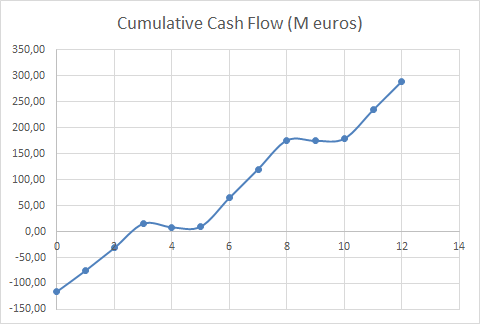
\includegraphics{CCF.png}

From the shown graphic and also from the table, it can be seen that between years 2 and 3, the Cumulative Cash Flow goes from a negative value to a positive one. Therefore, the Pay Back Time is between those two years. This gives a rough approximation of when will the investment be recouped. To be more precise about it, it can be linearly interpolated:

\begin{equation}
\frac{19.18-(-27.37)}{3-2}=\frac{19.18-0}{3-x}
\end{equation}

Solving for x, the result is of a PBT of 2.59 years.

In year 4, the satellites that are going to be launched in year 5 are made. This means an increase in the cost, due to the fabrication and assembly. Moreover, in year 5, there is also a increase, even more significant, because of the re-launching itself of those satellites. This is what causes that interval of time in which the Cumulative Cash Flow does not increase, but even decreases a bit: that year, the income is slighly smaller than the re-launching costs. This is why the Cumulative Cash Flows decreases a bit.

In years 9 and 10, the same process takes place again: the fabrication and re-launching of the new satellites. Nevertheless, profit is high enough at this point so that the Cumulative Cash Flow does not get to negative values again. 

The value of the first PBT (2.59 years) found seems reasonably acceptable, taking into account that this project requires a great budget, as all space projects do, due to its own nature. 




\subsection{Updated Pay Back Time (UPBT)}
Again, the Discounted Cumulative Cash Flow can be plotted as follows:

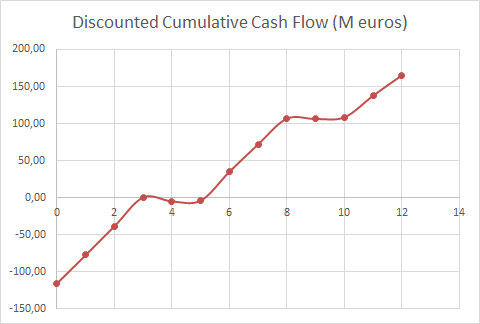
\includegraphics{DCCF.png}

The discount rate that has been considered is of a 6\% anual. It can be seen that between years 2 and 3, this value goes from a negative value to a positive one. Thus, the Updated Pay Back Time is between those two years. It can be linearly interpolated to gain some precision:

\begin{equation}
\frac{4.62-(-34.47)}{3-2}=\frac{4.62-0}{3-x}
\end{equation}

Solving for x, the result is of a UPBT of 2.88 years.

This time, because of the significat costs during year 4 (building and assembling of satellites) and especially year 5 (re-launching of satellites), added to the fact that the discount rate is now being taken into account to, it makes the Discounted Cumulative Cash Flow negative again, as can be seen in the graphic. Therefore, there will be another Updated Pay Back Time for the inversion done during years 4 and 5. It might be interesting to find it. It can be seen that it will be between years 5 and 6. Interpolating again:

\begin{equation}
\frac{0.19-(-0.69}{5-4}=\frac{0.19-0}{5-x}
\end{equation}

Solving last time for x, the result if a second UPBT of the year 4.79. Taking into account that this inversion was made during the year 4, it turns out to be an actual UPBT of 0.79 years.

There won't be a third UPBT. In years 9 and 10 there is a big investment again, but by then, the profit is high enough so as to make it possible for the Discounted Cumulative Cash Flow to not become negative any more. 

Again, that first value of UPBT (2.88 years) seems reasonably acceptable, because of the nature of the project, within the space sector, a very demanding and expensive one. The second investment required will also have a Updated Pay Back time, in this case of 1.10 years. It is smaller because the investment is not as high as the initial one, and there is already being great benefit. 

\subsection{Break Even Point (BEP)}
The Break Even Point is the point at which total cost and total revenue are equal, there is no net loss or gain. This figure represents the sales amount (quantity) required to cover total costs, consisting of both fixed and variable costs to the company. At this point, the total profit is zero. 

In Astrea's case, the Break Even Point is the number of Mbits sold the first year so that the Cash Flow of that year is just 0 (or approximately). 

By changing manually the parameter "Number of Mbits hired" of first year, it is found that the Break Even Point is of 49500000 Mbits (with this value of Mbits hired the first year, the Cash Flow is approximately 0). This means that under no account there can be less Mbits hired, otherwise, the Cash Flow would be negative and the Cumulative Cash Flow, negative at beginning since first year is fully just invest, would never reach a positive value, generating losses. 

From the assumptions of demand already explained, it can be seen that having a greater demand than the BEP is very likely to happen. Thus, the cash flow will be positive and consequently there will be a time in which there is benefit.

\subsection{Net Present Value (NPV)}
From the table, it can be immediately seen that the Net Present Value (for the period of time studied, of 12 years) is of +169.32M\euro. The Net Present Value is the difference between the present value of cash inflows and the present value of cash outflows over a period of time. It is clearly positive, which indicates that the project earnings generated by the investment exceeds the costs. In other words, it will be profitable. The Net Present Value coincides with the value of the Discounted Cumulative Cash Flow of the twelfth year. 


\subsection{Internal Rate of Return (IRR)}
The internal rate of retorn is the interest rate at which the Net Present Value of all the cashflows is equal to zero. This is used to evaluate the attractiveness of a project. If the Internal Rate of Return of a project exceeds a company's required rate of return, the project is desirable, and if on the other hand the IRR falls below the required rate of return, the project should be rejected.

The studied carried on uses a 6\% as the discount rate, and this value gives a positive Net Present Value, as has been already explained. By manually changing the discount rate, it can be achieved that the Net Present Value gets to 0, or very closely. This value of the discount rate is the Internal Rate of Return, and is used to evaluate the attractiveness of a project. In this case, it has been found that the IRR is of 29.15\%. The higher the IRR is, the more desirable is to undertake the proeject. In any case, it must be greater than the actual discount ratio. In this case, not only the IRR is greater, but it is actually a very high rate. Therefore, the project is very attractive, feasibly speaking. 

\subsection{Conclusions of the feasibility study}
It has already been seen that the Pay Back Time and the Updated Pay Back Time are both between 2 and 3 years. Taking into account that the space sector is a very exclusive one, in which the investment required is massive, those two parameters seem to be quite reasonable, indicating that the time required to recoup the funds expended in the investment is of less than 3 years. Moreover, since in years 4 and 5 there is again another investment because of the fabrication and re-launching of the satellites, there is a second Updated Pay Back time, in this case of roughly 1 year from the time the investment is done.

Regarding the Break Even Point, it has been determined that the amount of Mbits needed to make cost equal to total revenues is much smaller than the actual demand of data expected. Therefore, the cash flow will be positive and thus there will eventually profit.

Finally, analysing the Net Present Value and the Internal Rate of Return, the first one is positive and considerably big, and the secon one is greater than the actual discount ratio. This means that the investment is very likely to provide a good financial result.

As a final conclusion for this study, it has been clearly seen that the project is economically feasible. Nevertheless, it must not be forgotten than this study is done upon some important assumptions, which provide a certain degree of uncertainty. Nonetheless, the results of the study have been so positive that a slight variation of the hypothesis done could not lead to a unfeasible situation. 



\chapter{Marketing Plan}
\section{Executive Summary}
Astrea is the result of an enormous amount work and effort from its 17 co-founders and its name needs to be spread all over the world in order to start selling its services. In order to do that it is important to define the target customers to whom the service offered is going to be sold. Being the latter clear, it's essential to point out what does Astrea offer that makes it stand out from the rest of companies in the sector, that is, making an assessment of the strong points of the company. Moreover, it is necessary to establish the price at which the service is going to be sold to the customers and defining the position of the company among its competitors in the sector.
\newline\newline
Of course none of the above would make sense without defining a distribution plan in which the way customers buy from us is defined. In addition to that, the marketing materials used also have to be defined along with the online marketing strategy.
\newline\newline
A conversion strategy has to be defined too, that is, defining a way to turn prospective customers into paying ones. Finally, possible partnerships or future partnership plans will be assessed.
\section{Target Customers}
One of the most important items when it comes to selling a product or service is to whom it may be of interest. Since the service sold is essentially a communication bridge between satellite-to-satellite, Earth-to-satellite or Earth-to-Earth, it is well obvious that the average customer is not going to be an average consumer.
\newline\newline
Instead the service offered is projected towards public or private institutions such as aerospace universities who would like to execute experiments which require a reliable communication between their own spacecraft and their ground stations. Also towards start-up enterprises who would like to enter into the aerospace industry and need Astrea's infrastructure to accomplish their own projects.
\newline\newline
In addition to all of the above, the service is also targeted towards space agencies who plan on doing pilot missions with which Astrea could help with. Also aerospace enterprises who nonetheless would like to test their technologies and need real time feedback from them. Finally another targeted sector would be the communications enterprises who would like to acquire real time information from Earth's surface or outer space.
\section{Unique Selling Proposition}
The USP is, as the title appoints, what Astrea has to offer that sets it apart from other companies in its sector. Everyone in Astrea knows what the company is capable of and what it can offer and this is no more and no less than:
\begin{itemize}
\item Global signal coverage: Astrea's constellation covers every single spot on Earth's surface. This means that every ground station will have full-time signal coverage.
\item Ground station support: Astrea offers ground stations to its customers. For advanced users, custom ground stations are also available.
\item High reliability: Astrea's constellation is robust. Therefore, reliability is guaranteed.
\item Cheapest price on sector: Astrea brings global communication to customers at the lowest and most affordable price.
\end{itemize}
\section{Pricing \& Positioning Strategy}
The communication service Astrea offers is set to a price of 0.1\euro /Mb. Since there are no other companies offering the same kind of service it is not possible to make a comparison as of now. 

\section{Distribution Plan}
Since what Astrea offers is not a conventional service, people will not be able to purchase it directly. Instead, we use our website to get people to know what Astrea does as well as a way for our customers to get in touch with us. When a customer contacts us we provide them with all the necessary information on how to properly use our systems. Once the contract is made they can start using our communication systems right away. The payment is done monthly much like a regular mobile carrier. Customers will get their invoices with their total data consumption and price.

\section{Marketing Materials}
The marketing materials we count on are:
\begin{itemize}
\item A website: http://astrea.upcprogram.space/
\item An informative and encouraging video.
\item Brochures.
\item A poster.
\end{itemize}

\section{Online Marketing Strategy}
Given the fact that our distribution plan is executed in an essentially online manner, it makes sense to elaborate an Online Marketing Strategy. The key components to our online marketing strategy are:
\begin{enumerate}
\item Keyword Strategy: it is important to identify the keywords to optimize our website for. In our case the keywords would be: "Astrea", "constellation", "reliability", "CubeSat" and "communication".
\item Search Engine Optimization: document updates will be made to the website in order to appear more prominently in online search engines.
\item Social Media Strategy: nowadays it is crucial to be in the social media. The world is permanently connected through the social media and it can be one of most powerful ways to show off what we've produced. Therefore, Astrea will have its own Twitter, Instagram and Facebook accounts.
\end{enumerate}
\section{Conversion Strategy}
The technique we use to turn prospective customers into actual paying customers will be showing testimonials from actual customers who were satisfied with our service in our website. In addition to that, we will post in our website every successful project we provide service to. This will show the reliability of the service to the insecure customers and hopefully turn them into actual customers
\section{Joint Ventures \& Partnerships}
Right at its beginning Astrea does not count on any Joint Ventures nor Partnerships with other enterprises. Nevertheless, Astrea is open to future partnerships with businesses who would like to work in collaboration with us.




\chapter{Environmental Impact Study}
\section{Introduction}
This chapter pretends to assess the environmental consequences (positive and negative) of developing the project. The target of this study is to identify, predict, evaluate and mitigate the biophysical and social negative effects that the project could generate during the execution of it.
\section{Ground Stations}
At first sight the Ground Stations do not represent any environmental problem. The main factor that has to be taken into account is the placement of the stations. They have to be located in a place where they do not interfere with the ecosystem. The placement of the stations has to be adequate with the environmental legislation of the countries. 
\section{Satellites}
For analysing the impact of the satellites it has to be studied the possible environmental impact during the fabrication and during the orbital life.
The fabrication of the satellite components is externalized, and they are bought as products of these companies. All this products have been tested and checked, complying all regulations. The fabrication of these products does not involve an environmental damage. 
During the orbital performance of the satellites, it has to be taken into account whether or not they would become orbital waste. The satellites are designed to burn out in the atmosphere at the end of their useful life. This burnt should not leave any solid residue that could precipice over the surface. The deorbit would be forced and controlled by the propulsion system of the satellite. In the case that this system fails, given that they will orbit in a LEO, they will be deorbited and burnt out naturally in a period around 5 years.
\section{Launch system}
The most critical part of the entire process, in environmental terms, is the launch of the satellites. For this reason the main relevance in this report is given to the spacecraft that will put the satellites in orbit, the Electron rocket of Rocket-Lab.
The company operate in New Zeeland, and for doing it, the Ministry for the Environment make an accurate study of the environmental impact of the Electron launching. The entire document can be seen at \cite{EIS}.
In this document are analysed the critical components of the spacecraft:
\begin{itemize}
\item \textbf{Structure}. The primary structural material is carbon fibre reinforced polymer. The carbon filaments are chemically inert and do not react to seawater.
\item \textbf{Propellants}. Liquid oxygen and kerosene (RP-1 analogue) propellants are used on both the first and second stages of the launch vehicle. Liquid oxygen, if released to the atmosphere, rapidly boils and returns to the atmosphere as gaseous oxygen. RP-1 kerosene is a highly refined grade of hydrocarbon with low density, a thin surface film and rapid evaporation.
\item \textbf{Pneumatics}.All inflight pneumatic systems use stored pressurised cold gases to provide tank pressurisation, cold-gas manoeuvring thrust in space, and for stage separation mechanisms. All gases are non-toxic.
\item \textbf{Engines}. The launch vehicle uses nine engines for stage 1 and a single engine for stage 2. The engines are constructed of inconel, an inert high performance, corrosion resistant nickel alloy. At stage 1 separation, the thrust section is likely to separate from the stage, return to Earth’s surface and land in the Exclusive Economical Zone.
\item \textbf{Batteries}. The first stage batteries are highly likely to burn-up before returning to Earth’s surface. The stage 2 batteries will entirely burn-up downrange, with only the first battery potentially landing in the EEZ. The batteries are lithium-based, and contain no lead, acid, mercury, cadmium, or other toxic heavy metals.
\end{itemize}
The document also evaluates the following possible risks:
\begin{itemize}
\item \textbf{Risk of toxic effects}. The toxic effects of the materials comprising stage 1, the fairings and the two stage 2 LithiumIon batteries were assessed as low at all levels of launch activity.
\item \textbf{Risk of ingestion of materials and provision of floating shelter}. Floating jettisoned materials as shelter for pelagic organisms and the ingestion of jettisoned materials were both evaluated as having low ecological risk at all levels of launch activity.
\item \textbf{Environmental effect of the displacement of fishing activities.} For the demersal fish
and mobile invertebrate community, marine mammals and seabirds, the effects of fishing displacement would be low because these populations could also be impacted in the areas to which fishing is displaced. In the eastern jettison zone there is less fishing activity so the consequences of fishing displacement on the seabed community, demersal fish and mobile invertebrates, marine mammals and seabirds are negligible, reaching minor impacts after 1000 or more launches.
\item \textbf{Effect of the provision of hard substrates.} Another potential positive outcome for seafloor biota requiring hard substrates is that the jettisoned materials would provide further attachment sites. However, even after 10,000 launches this would provide only about 50 ha of additional attachment surface, leading to a moderate benefit at most.
\item \textbf{Disturbance to marine fauna.} Noise and disturbance to marine fauna above and below water is a potential consequence of
the jettisoned materials falling into the jettison zone. The chance of repeated disturbance to the same individuals or groups of marine mammals or seabirds increases with the number of launches. This was assessed as a low risk for up to 100 launches over two years, a moderate risk for up to 1000 launches over almost 20 years, and a high risk for up to 10,000 launches over almost 200 years.
\item \textbf{Risk of direct strikes causing mortality to components of the ecosystem.} Direct strikes causing mortality are a low risk for all components of the ecosystem up to 1000 launches over an almost 20 year period. Direct strikes reach moderate levels of risk for the benthic invertebrate community, sensitive benthic environments, and a rare threatened species, the magenta petrel, after 10,000 launches over a period of almost 200 years.
\item \textbf{Risk of smothering of sea floor organisms.} Smothering the feeding or respiratory structures of sea floor organisms by jettisoned materials was assessed as a low risk for all levels of launches up to 1000 launches and a moderate risk by 10,000 launches. This is likely to be a factor principally in areas of hard substrate where the jettisoned materials are unlikely to become buried in sediment so will be important principally on the Bounty Platform.
\end{itemize}
New Zealand legislation does not yet regulate these activities, since Rocket Lab is the first company that pretends to operate rocket launchings in the territory. The study concludes that the environmental effects of the activity may become significant after 10,000 launches, this would take 200 years to reach at one launch per week. The regulatory regime would have been reviewed well before this number of launches. During this review the Ministry allows the activity of the company.

\chapter{Social and Security Considerations}

\section{Social and security considerations}

The potential of the CubeSats is very high and they might be the future of satellites. Their low cost and the easiness to construct them, compared to large satellites, make them accessible to countries with fewer resources, universities and people in general, making them able to explore the space and to pursue different missions. The assembly of a CubeSat is not very complicated but requires a minimum knowledge about the subject; in other words, now "you've got a user manual, a datasheet and a 3D model that you can download, and you've got an online shop where people can buy their power systems, etc with their credit card" \cite{CraigClark}. 

This project is based on the design of a satellite constellation dedicated to communications relay between LEO satellites and between LEO satellites and the ground. This project is helping to develop the CubeSat industry and its use and it will demonstrate that these small satellites can carry out different missions that were previously done only by large satellites, as for example the communication.

Currently, the constellations of CubeSats dedicated to the communication are in development and the market is not very extensive, this is why this project, and the global coverage that it provides, could have a privileged place in this industry. The main commitment that this project has with the customers is to ensure that they will be able to communicate with any part of the world without problems. 

Another important aspect to consider is that the constellation will provide total privacity  to the costumers, ensuring that they make a correct use of it and avoiding that third people interfering in the communication.

In relation to security, it must ensured the proper functioning of the constellation. To do this, it must be considered three main factors, where CubeSats could be in danger: the launch of the payload, the permanence of the CubeSats in space and the ground stations.

The launch stage is one of the most important, because it is where the mission has more probability to fail. In the next figure can be observed the succes rate of orbital launches in the last 57 years. In 2014, there were a total of 92 unmaned launches and only 4 of them were failed. This indicates that the fail rate is only a 4,34 \%, which is very low. 

\pagebreak

\begin{figure}[h!]
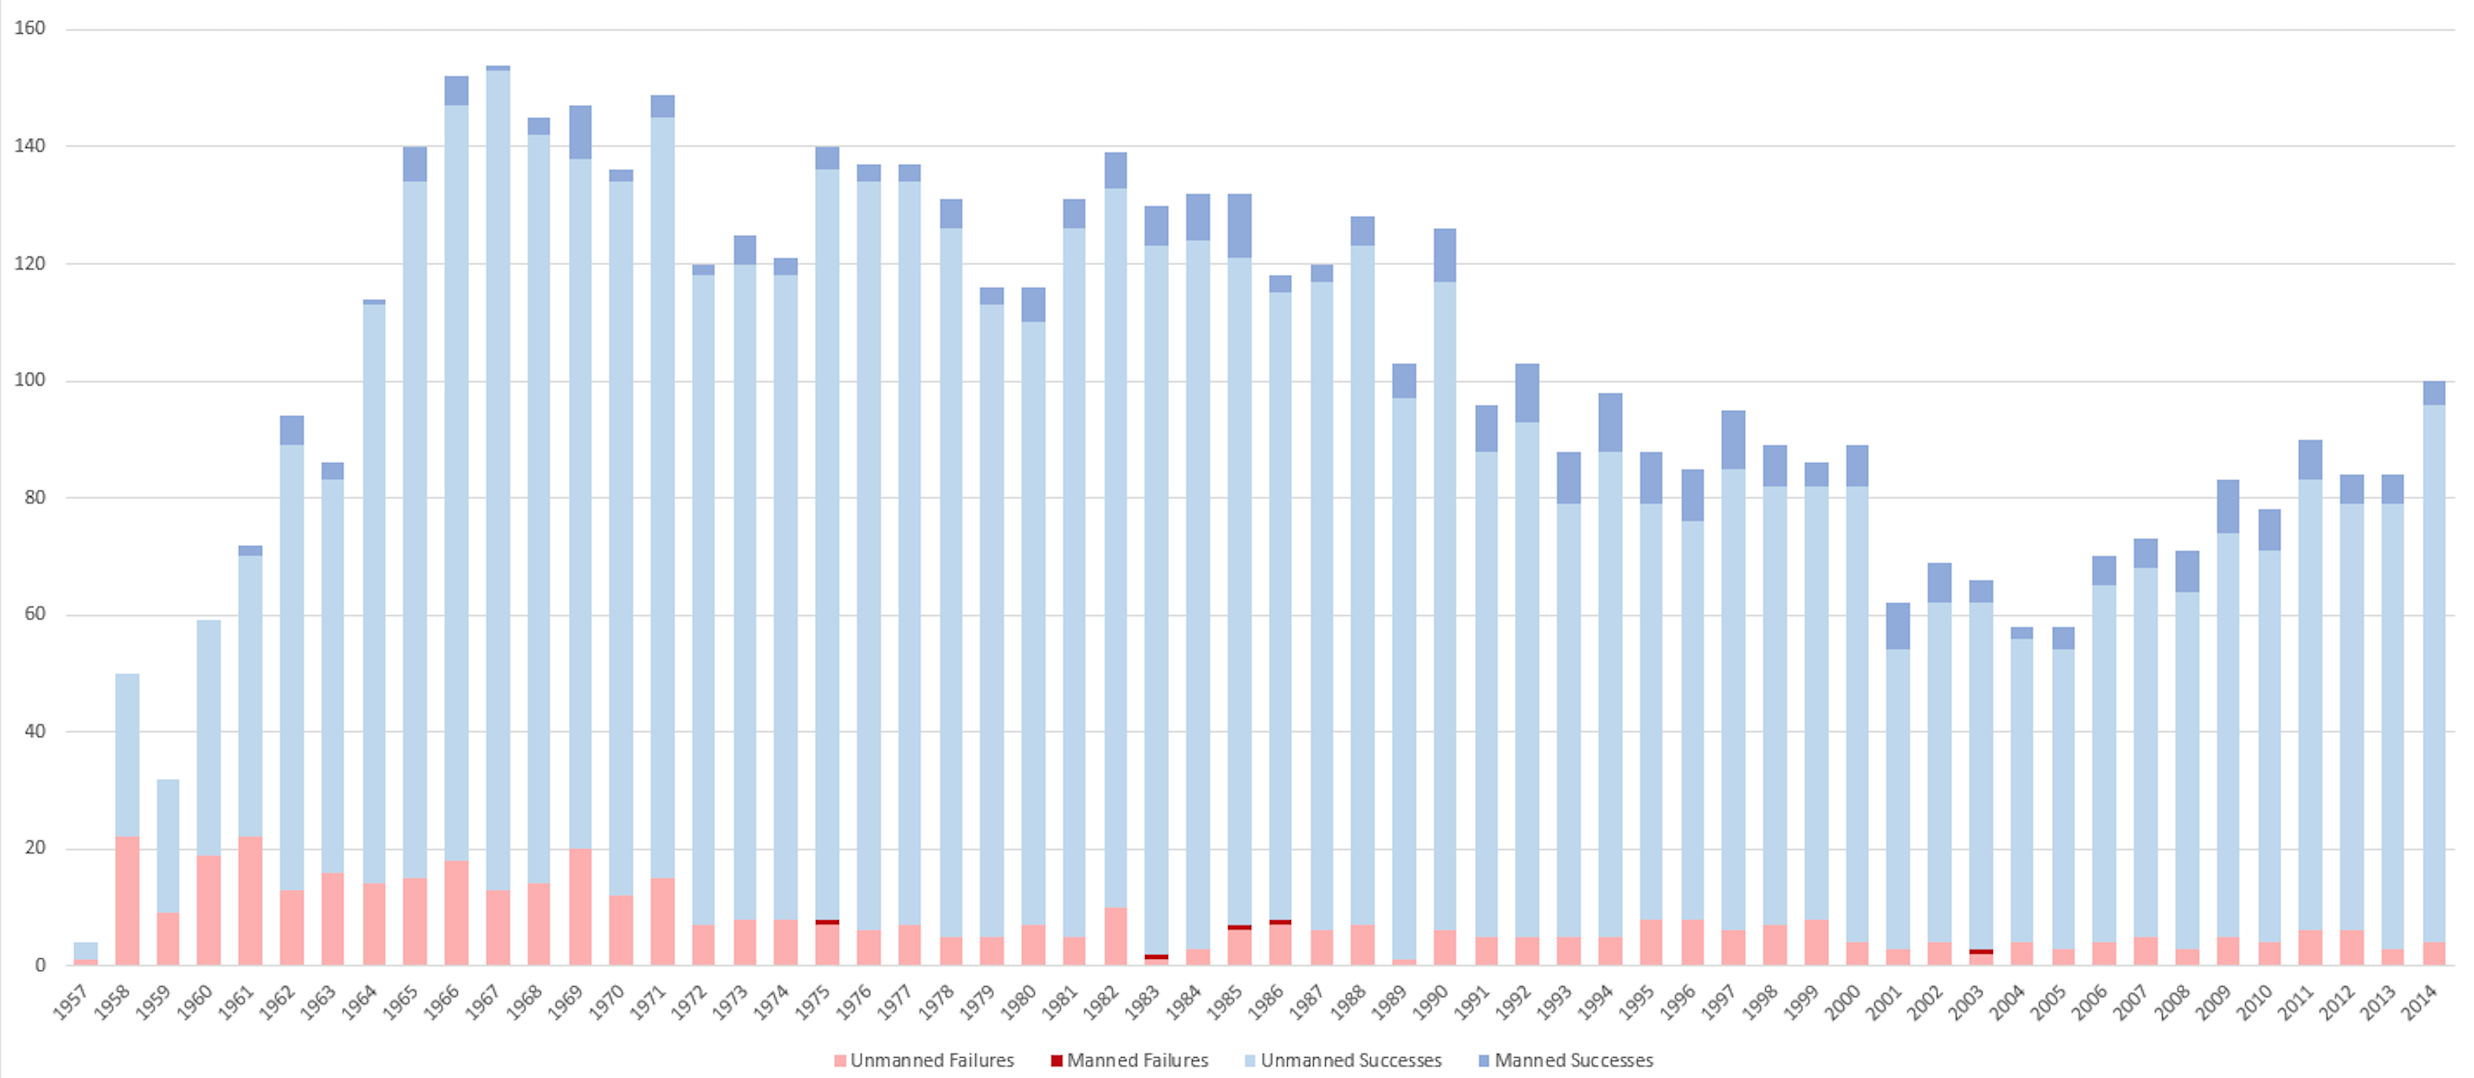
\includegraphics[scale=0.3]{./OrbitalSummary}
\centering
\caption{Orbital Launch Summary by Year}
\end{figure}

\paragraph{}Once the constellation is in orbit, CubeSats can find dangers how colliding with other satellites or with space debris. The distances between most satellites is around hundreds of miles and there is not danger of collision, but the movement of space debris is unpredictable. In order to avoid this space debris, a CubeSat can perform a Debris Avoidance Manoeuvre (DAM). The responsible to control these fragmentation debris is \textit{The United States Space Surveillance Network}. It consists of ground-based radars and optical sensors at 25 sites worldwide and Currently tracks more than 8000 orbiting objects.

Finally, the ground stations are a key element for the correct operation of the constellation and they must prevented from stop working. To do this, each ground station will have its operator, to control the operation of the installation, and a security system, to avoid intrusions.

\section{Legislation}
The legislation concerning activities related to space is the Space Law. Space Law is an international law comprised of international treaties and agreements. Its most important rules are the five international treaties, which have been developed under the supervision of the United Nations. The body that promotes these regulations is the United Nations Office for Outer Space Affairs (UNOOSA).
\newline
\newline
The international law is only applicable to the states that are parties to the treaties. According to the Outer Space Treaty, states are responsible for their national space activities, public or private. For this reason, each state usually adopts its national space regulations.
\newline
\newline
In the case of the Astrea constellation, since the company is based in Spain (a party of the Space Law), the current legislation is the \textit{Real Decreto 278/1995} of 24 February 1995. According to this Royal Decree, the objects launched from Spain or whose launch has been promoted by Spain, should be registered in the \textit{Registro Español de Objetos Espaciales Lanzados al Espacio Ultraterrestre} (Spanish Registry of Objects Launched into Outer Space). The necessary data to register the satellite must be provided to the \textit{Dirección General de Tecnología Industrial del Ministerio de Industria y Energía} (Department of Industrial Technology of the Ministry of Industry and Energy). This department will notificate the registry to the Secretary-General of the United Nations.
\newline
\newline
The registration has to contain the following data:
\begin{enumerate}[label=\alph*)]
\item Name of launching State or States;
\item An appropriate designator of the space object or its registration number;
\item Date and territory or location of launch;
\item Basic orbital parameters, including:
\begin{enumerate}[label=\Roman*)]
\item Nodal period;
\item Inclination;
\item Apogee;
\item Perigee;
\end{enumerate}
\item General function of the space object.
\end{enumerate}
and any other useful information.
For example, in the case of one of the Astrea satellites, the registration will be:
\begin{enumerate}[label=\alph*)]
\item Spain
\item AstreaSAT 1
\item 22 February 2018, 
\item Basic orbital parameters: Low Earth Orbit
\begin{enumerate}[label=\Roman*)]
\item 95,4815 minutes
\item 72 degrees
\item 6.913,0 km
\item 6.913,0 km
\end{enumerate}
\item CubeSat 3U, part of the communications constellation Astrea
\end{enumerate}
